% IEEE SP Cup 2027 (FaceVitals), Round 1 technical report -- DRAFT
%
% Build:   tectonic main.tex        (or upload this folder to Overleaf)
% Numbers: every table is generated by report/stats.py from saved results
%          (report/tables/*.tex, report/figs/*.pdf, report/numbers.json);
%          numbers quoted in the text come from report/numbers.json.
%
% Search for \pending{ to find everything the team still has to fill in.
\documentclass[conference]{IEEEtran}
\IEEEoverridecommandlockouts
\usepackage[T1]{fontenc}
\usepackage{cite}
\usepackage{amsmath,amssymb}
\usepackage{graphicx}
\usepackage{booktabs}
\usepackage{array}
\newcolumntype{L}[1]{>{\raggedright\arraybackslash}p{#1}}
\usepackage{xcolor}
\usepackage{tikz}
\usetikzlibrary{positioning,arrows.meta}
\usepackage[hidelinks]{hyperref}

\newcommand{\pending}[1]{\textcolor{red}{\textbf{[TO DO: #1]}}}
\newcommand{\bpm}{\,bpm}
% \input is not expandable in current LaTeX, which breaks \bottomrule after it in a tabular.
\makeatletter\newcommand{\tablerows}[1]{\@@input #1 }\makeatother

\begin{document}

\title{Codec-Aware, Quality-Gated Heart-Rate Estimation\\from Low-Quality Facial Video}

\author{\IEEEauthorblockN{\pending{Author 1}, \pending{Author 2}, \pending{Author 3}, \pending{Author 4}}
\IEEEauthorblockA{\pending{Department, University, City, Country}\\
\pending{email addresses} \quad Supervisor: \pending{name}}}

\maketitle

\begin{abstract}
We present a real-time heart-rate (HR) estimator for RGB facial video, designed around the deployment
constraints of the 2027 SP Cup. A target-locked face front end samples six skin patches, the whole face
and the background. The colour traces are cleaned of video-codec and illumination artefacts, turned into
pulse spectra by the POS algorithm and by a 27k-parameter temporal CNN, fused by signal-to-noise ratio
and tracked with a Viterbi decoder. A quality gate estimates, for every window, the probability that the
error is within 5\bpm, and withholds readings below 0.8. We identify the main failure under the
10\,fps / 500\,kbps constraint: the B-frame cycle of default H.264 encoders puts a colour artefact at
exactly 150\bpm. We remove it at both the sender and the receiver. The system was developed on 60 subjects
of the public MCD-rPPG dataset and tested once on 20 subjects never used in development. Under normal
conditions it reaches a mean absolute error (MAE) of 1.49\bpm{} ($r=0.95$), against 5.84\bpm{} for POS. It
stays at or below 2.4\bpm{} at QVGA resolution, at simulated 50 and 20\,lux, with a bystander in frame, and
when streamed at 10\,fps and 500\,kbps with our sender settings. In every condition, 94--98\,\% of the reported windows are within
5\bpm. Simulated surgical masks remain the main weakness (8.6\bpm); the system detects them and
withholds most of those windows. Without retraining, on the UBFC-rPPG dataset (another lab, camera and
lighting; 42 subjects) the MAE is 0.85\bpm{} under normal conditions and at most 0.95\bpm{} under
simulated low light, low resolution, bystanders and masks; low-bandwidth streaming is harder there
(3.2\bpm{} with our sender).
\end{abstract}

\begin{IEEEkeywords}
remote photoplethysmography, heart rate, video compression, low light, signal quality, abstention
\end{IEEEkeywords}

\section{Introduction}
Remote photoplethysmography (rPPG) recovers the blood-volume pulse from small colour changes of facial
skin~\cite{verkruysse2008,poh2010}. Under good conditions, simple projection methods such as
CHROM~\cite{dehaan2013} and POS~\cite{wang2017} already track HR well. The FaceVitals challenge asks for
more: HR from consumer cameras in low light, at low resolution, over 10\,fps / 500\,kbps links, with
bystanders and masks, and with honest validation against a contact reference. Each of these conditions
breaks a different assumption of the classical pipeline, and a method that only reports a pooled error
hides where it fails.

This report describes our Round~1 system and how we evaluated it. Our contributions are:
\begin{itemize}
\item \textbf{A diagnosis of the low-bandwidth failure (C5).} With default H.264 settings, every
fourth frame starts a new P\,B\,B\,B group; each position in the group is quantised differently, and at 10\,fps this
cycle is a 2.5\,Hz (150\bpm) colour oscillation inside the HR band. Uneven frame decimation and the
face-mesh refresh rate add further errors. We fix these at the sender (no B-frames, fixed decimation)
and at the receiver (phase regression), without tuning on test data.
\item \textbf{A hybrid estimator.} A 27k-parameter temporal CNN learns colour and region mixing from
the traces and is fused with POS in the spectral domain. Out-of-fold, this cuts the error by 43--64\,\% in every
unmasked condition.
\item \textbf{Quality-gated reporting.} A small classifier predicts, per window, whether the
error is within 5\bpm. Readings below a fixed threshold are flagged rather than reported, so that 94--98\,\%
of reported windows are within 5\bpm{} in every tested condition.
\item \textbf{A strict evaluation protocol.} Every number comes from subjects the scoring models
never saw: subject-disjoint cross-validation for development, then two held-out sets, each scored
only once, and a cross-dataset test on UBFC-rPPG with nothing retrained. We also report an ablation of
every stage and results by skin tone, age and sex.
\end{itemize}

\section{Related Work}
Classical rPPG separates the pulse from specular and motion components by colour projections
(CHROM~\cite{dehaan2013}, POS~\cite{wang2017}) or by blind source separation~\cite{poh2010}. Li
\textit{et al.}~\cite{li2014} used a background region to rectify illumination changes; our
illumination step is a closed-form, per-window version of that idea. Deep models learn the projection
from data, either from frames~\cite{chen2018deepphys,yu2019physnet,liu2023efficientphys} or from
pre-extracted traces; rPPG-Toolbox~\cite{liu2023toolbox} collects many of them. McDuff \textit{et
al.}~\cite{mcduff2017} showed that compression degrades rPPG, but did not analyse the effect of the
B-frame cycle at low frame rates. Nowara \textit{et al.}~\cite{nowara2020} found larger errors for
darker skin, which motivates C2 and our stratified reporting. Our quality gate is a form of selective
prediction~\cite{geifman2017}: trading coverage for reliability.

% --------------------------------------------------------------------------------------------
\begin{figure*}[t]
\centering
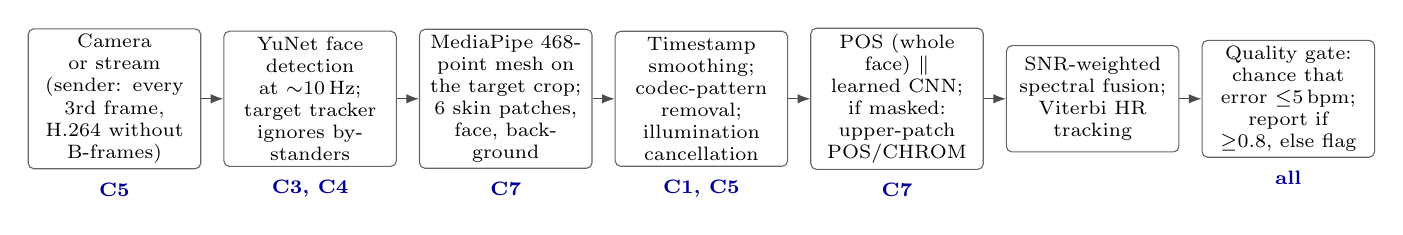
\begin{tikzpicture}[
  box/.style={draw=black!60, rounded corners=2pt, align=center, font=\scriptsize,
              minimum height=1.35cm, text width=2.05cm, inner sep=2pt},
  tag/.style={font=\scriptsize\bfseries, text=blue!60!black},
  arr/.style={-{Latex[length=1.6mm]}, black!70}]
\node[box] (cam) {Camera or stream\\ (sender: every 3rd frame, H.264 without B-frames)};
\node[box, right=0.28cm of cam] (det) {YuNet face detection at $\sim$10\,Hz;\\ target tracker ignores bystanders};
\node[box, right=0.28cm of det] (roi) {MediaPipe 468-point mesh on the target crop;\\ 6 skin patches, face, background};
\node[box, right=0.28cm of roi] (clean) {Timestamp smoothing; codec-pattern removal; illumination cancellation};
\node[box, right=0.28cm of clean] (pulse) {POS (whole face) $\|$ learned CNN;\\ if masked: upper-patch POS/CHROM};
\node[box, right=0.28cm of pulse] (track) {SNR-weighted spectral fusion;\\ Viterbi HR tracking};
\node[box, right=0.28cm of track] (gate) {Quality gate: chance that error ${\le}5$\,bpm; report if ${\ge}0.8$, else flag};
\foreach \a/\b in {cam/det, det/roi, roi/clean, clean/pulse, pulse/track, track/gate} \draw[arr] (\a) -- (\b);
\node[tag, below=0.05cm of cam] {C5};
\node[tag, below=0.05cm of det] {C3, C4};
\node[tag, below=0.05cm of roi] {C7};
\node[tag, below=0.05cm of clean] {C1, C5};
\node[tag, below=0.05cm of pulse] {C7};
\node[tag, below=0.05cm of gate] {all};
\end{tikzpicture}
\caption{Processing pipeline. Labels show the constraints each stage addresses.}
\label{fig:pipeline}
\end{figure*}

\section{Method}
Fig.~\ref{fig:pipeline} shows the pipeline. It runs both offline (recorded video) and online
(webcam or stream), and the same code is used for both.

\subsection{Face front end and regions of interest}
YuNet~\cite{wu2023yunet} detects all faces at half resolution about 10 times per second (every third
frame at 30\,fps, every frame at 10\,fps). A target tracker keeps one designated face. The target is
chosen at start-up (the largest face, or the face nearest a selected point); after that, each detection
round takes the box with the highest IoU ($>0.3$) with the target's constant-velocity prediction. After
more than five missed rounds it re-acquires only a face close to the last target position, so it never
switches to a bystander. The MediaPipe face mesh~\cite{kartynnik2019} (468 landmarks) then runs on the target crop only,
which keeps its cost independent of the number of people in view. From the mesh we sample the mean RGB
of six skin patches (forehead, glabella, both malar cheeks and both lower cheeks), the whole face oval,
and two background boxes beside the face at eye level. Saturated and black pixels are excluded.

\subsection{Trace conditioning}
\textit{Timestamps.} Traces are placed on the real capture times. The webcam's logged stamps come in
${\sim}16$\,ms timer steps, so we remove this jitter by averaging each stamp's deviation from a constant
frame period over ${\sim}1$\,s, which keeps genuine drift and dropped frames. The traces are then
resampled to a uniform 30\,Hz grid.

\textit{Codec-pattern removal.} Let $\phi(n)$ be the number of frames since the last I or P frame
(read from the stream). For each region and channel, the normalised trace $\tilde c(n)=c(n)/\mu-1$ is
high-passed with a moving average spanning whole cycles. It is then regressed on the zero-mean phase
indicators $\mathbf{D}=[\mathbb{1}\{\phi(n)=k\}]_{k\ge1}$, and the fitted offsets $\mathbf{D}\boldsymbol{\gamma}$
are removed from $\tilde c$. A stream without B-frames has a single phase and is left unchanged.

\textit{Illumination cancellation.} Flicker, its aliases at low frame rates, and global light changes
modulate skin and background alike, but only skin carries the pulse. With $\mathbf{B}$ the band-passed,
normalised background RGB ($N\times3$), each skin region becomes
\begin{equation}
\hat{\mathbf c}_r=\tilde{\mathbf c}_r-\mathbf{B}\boldsymbol{\beta}_r,\qquad
\boldsymbol{\beta}_r=\arg\min_{\boldsymbol\beta}\big\|\mathcal{H}\tilde{\mathbf c}_r-\mathbf{B}\boldsymbol\beta\big\|^2,
\end{equation}
where $\mathcal H$ is a third-order Butterworth band-pass over 0.66--3.5\,Hz (40--210\bpm).

\subsection{Pulse spectra}
\textit{Classical branch.} POS~\cite{wang2017} (1.6\,s overlap-add windows) is applied to the whole-face
trace. GREEN and CHROM~\cite{dehaan2013} are computed as well, but only as evidence for the quality gate.
For each 10\,s window (1\,s hop), a Hann-tapered DFT gives the power $P(f)$ on a 1\bpm{} grid from 40 to
200\bpm.

\textit{Learned branch.} A temporal CNN takes 27 input channels per 10\,s window. For each of the eight
regions it receives the mean-normalised, band-passed RGB; it also receives the whole-face POS, CHROM and
GREEN signals. It has a $1{\times}1$ input layer (32 channels), five residual blocks of dilated
convolutions (kernel 5, dilation 1--16, batch norm, ELU), dropout and a $1{\times}1$ output that emits a
pulse waveform (27\,073 parameters). It is trained with a spectral cross-entropy between the normalised
power of its output, $\hat P$, and a Gaussian ($\sigma=2.5$\bpm) centred on the contact-PPG heart rate:
\begin{equation}
\mathcal L=-\textstyle\sum_f \mathcal N(f;\,\mathrm{HR}_{\mathrm{PPG}},\sigma)\,\log \hat P(f).
\end{equation}
This loss ignores the pulse transit delay between face and finger. Training uses the full 3-minute
videos of the development subjects. Each video is time-stretched by factors 0.8--1.25 (with the label
scaled accordingly) so that high heart rates are better covered. Further augmentation flips the sign,
drops whole regions and adds noise. Training uses AdamW with a one-cycle schedule for 4000 steps and
takes about 2\,min on a laptop GPU.

\textit{Fusion and tracking.} Each spectrum is normalised to unit power and weighted by its
SNR~\cite{dehaan2013}: the power within $\pm6$\bpm{} of its own peak and $\pm12$\bpm{} of the second
harmonic, divided by the remaining power in the band. The fused spectrum is
\begin{equation}
\bar P_w(f)=\frac{\sum_k q_{k,w}\,P_{k,w}(f)}{\sum_k q_{k,w}},\qquad q_{k,w}=10^{\,\mathrm{SNR}_{k,w}/10}.
\end{equation}
A Viterbi decoder then finds the most likely HR path. Its emissions are $\log\bar P_w$, and its transitions are Gaussian
with $\sigma=3$\bpm{} per second plus a small floor, so that genuine jumps remain possible. The online
version runs the same recursion causally. We disabled the common harmonic boost: because the
band ends at 210\bpm, rates above 105\bpm{} can never earn it while their half-rate sub-harmonics can,
which biased the tracker toward half the true rate (Table~\ref{tab:ladder}).

\textit{Mask gate (C7).} A patch is marked occluded when its red-minus-blue chromaticity drops below
half of the forehead's, or when its chromaticity is far from the forehead's. When both lower cheeks are
occluded, the window switches from whole-face POS and the learned branch to SNR-fused POS and CHROM
spectra of the patches that still look like skin.

\subsection{Quality gate}
For every window we compute seven features: the SNR, the share of spectral power within $\pm4$\bpm{} of
the estimate, the gap between the tracker output and the spectral peak, the gap between the POS and
learned-branch peaks, the median power share over the surrounding 11 windows, and the gaps to the GREEN
and CHROM peaks. A gradient-boosted classifier (depth~3, 200 iterations) maps them to
$p_w=P(|e_w|\le5\,\mathrm{bpm})$. It is fitted on out-of-fold development windows; its AUC is 0.90 out-of-fold and 0.89 on the
held-out subjects. A window is reported if $p_w\ge0.8$; otherwise the HR is still output but flagged as low quality.
The threshold was fixed on the development subjects. Skin colour is deliberately not a feature.

\section{Experimental Setup}
\subsection{Data}
We use the public MCD-rPPG dataset~\cite{egorov2025} (CC\,BY\,4.0): 600 subjects, each recorded for
3 minutes at rest and again after exercise, with synchronised 100\,Hz contact PPG and ECG. We use the
frontal webcam (640$\times$480, ${\sim}30$\,fps). The reference HR is the spectral peak of the PPG in the
same 10\,s windows. For subjects that failed even under ideal conditions, we checked the reference by
beat counting and against the ECG.

Subjects are ordered by ID. The first 60 (120 videos; 36 female; ages 18--78, median 20; reference HR
47--136\bpm) are the \textit{development} set. All design choices were made on them with 5-fold
subject-disjoint cross-validation, so every development number is out-of-fold. Two \textit{held-out}
sets were each scored once, with everything frozen. The first, subjects 41--60, was scored with models
trained on subjects 1--40, before those subjects joined development. The second, subjects 61--80 (40 videos; 16 female;
ages 18--50; HR 52--120\bpm), was scored with models trained on subjects 1--60, and gives our headline
numbers. Evaluation uses the first 40\,s of each video (30 windows per video).

For a cross-dataset test we use UBFC-rPPG DATASET\_2~\cite{bobbia2019}, whose authors share 42 of its
46 videos. It was recorded in another lab with a Logitech C920 webcam (640$\times$480, uncompressed,
${\sim}30$\,fps) about 1\,m from the subject, indoors under varying sunlight and room light, while subjects
played a time-pressured maths game to raise their heart rate. The reference is a CMS50E transmissive pulse
oximeter, with one PPG sample per video frame. We use the whole videos (46--69\,s, median 68\,s), apply
the same constraint simulations, and compute the reference HR the same way. The reference HR spans
53--135\bpm{} (mean 98\bpm, against 81--85\bpm{} on MCD).

\subsection{Constraint simulations}\label{sec:sim}
All constraints are simulated on the same videos, which isolates each effect.
\textit{C1:} we undo the display gamma and scale the light by 50/300 or 20/300. We then draw Poisson shot
noise (full well 3000\,e$^-$) and Gaussian read noise (3\,e$^-$), apply auto-gain back to the original
brightness and quantise to 8 bits. This corresponds to the brief's ``combined degradation'' option.
\textit{C4:} we downsample to 320$\times$240 (the QVGA stress case) with area interpolation. Note that the
baseline is already VGA, below the 1280$\times$720 the brief specifies for Task~1.
\textit{C5:} we keep every third frame (30$\to$10\,fps) and encode with x264 at 500\,kbps (maxrate
500\,kbps, buffer 1000\,kb), both with default settings and with \texttt{zerolatency} tuning (our sender).
\textit{C3:} we place a second subject's video beside the target (1280$\times$480); the target is
designated once, at start-up.
\textit{C7:} we draw a light-blue textured surgical-mask polygon from the landmarks, from the mid nose
bridge to the chin. It covers 49\,\% of the face oval and 96\,\% of its lower half (the brief requires
${\ge}40$\,\%).

\subsection{Metrics}
Following the brief, we report the MAE, the RMSE, Pearson's $r$ and the Bland--Altman
bias with 95\,\% limits of agreement~\cite{bland1986}. All are computed over pooled 10\,s windows. We also report the share of windows
within 5\bpm{} and, with the quality gate, the coverage (the share of windows reported) and the error on
reported windows.

% --------------------------------------------------------------------------------------------
\begin{table*}[t]
\caption{Held-out results: subjects 61--80 (20 subjects, 40 videos, 1200 windows per condition), scored once
with models trained on subjects 1--60. MAE, RMSE and Bland--Altman (BA) values in bpm. ``Reported'' columns
apply the quality gate ($p\ge0.8$).}
\label{tab:heldout}
\centering
\footnotesize
\setlength{\tabcolsep}{3.4pt}
\begin{tabular}{lcccccccccc}
\toprule
 & \multicolumn{3}{c}{MAE, all windows} & \multicolumn{4}{c}{Proposed, all windows} & \multicolumn{3}{c}{Proposed, reported windows} \\
\cmidrule(lr){2-4}\cmidrule(lr){5-8}\cmidrule(lr){9-11}
Condition & POS & Classical & Proposed & RMSE & $r$ & BA bias [95\,\% LoA] & ${\le}5$\bpm{} (\%) & Reported (\%) & MAE & ${\le}5$\bpm{} (\%) \\
\midrule
\tablerows{tables/heldout.tex}
\bottomrule
\end{tabular}
\end{table*}

\begin{table*}[t]
\caption{Ablation on the development subjects (1--60, 120 videos), out-of-fold: each stage is added
in turn. Pooled MAE in bpm. The last two rows each change one design choice of the classical system.}
\label{tab:ladder}
\centering
\footnotesize
\begin{tabular}{lcccccccc}
\toprule
Stage & Normal & C4 QVGA & C1 50\,lux & C1 20\,lux & C3 bystander & C5 our sender & C5 default x264 & C7 mask \\
\midrule
\tablerows{tables/ladder.tex}
\bottomrule
\end{tabular}
\end{table*}

\section{Results}
\subsection{Accuracy on held-out subjects}
Table~\ref{tab:heldout} gives the headline results. Under normal conditions the proposed system has an
MAE of 1.49\bpm{} ($r=0.95$, Bland--Altman bias $+0.04$\bpm, limits $-7.6$ to $+7.7$\bpm), against
5.84\bpm{} for POS and 3.00\bpm{} for our classical branch alone. The system degrades gracefully: the
MAE stays at or below 2.4\bpm{} at QVGA, at simulated 50 and 20\,lux, with a bystander in frame, and
over a 10\,fps / 500\,kbps link with our sender settings. Fig.~\ref{fig:ba} shows the agreement plots.
On the earlier held-out set (subjects 41--60, model trained on subjects 1--40) the normal-condition MAE
was 2.65\bpm{} (classical 3.14, POS 5.87). That set has more fast, post-exercise heart rates, so results
should be compared between methods on the same set, not across the two sets.

With the quality gate, 73--85\,\% of windows are reported in every unmasked condition except default
x264 (65\,\%). The reported windows have an MAE of 1.2--2.2\bpm, and 94--98\,\% of them are within
5\bpm. The gate is most useful under masks: it reports 37\,\% of windows, and 97\,\% of those are
within 5\bpm.

\begin{figure}[t]
\centering
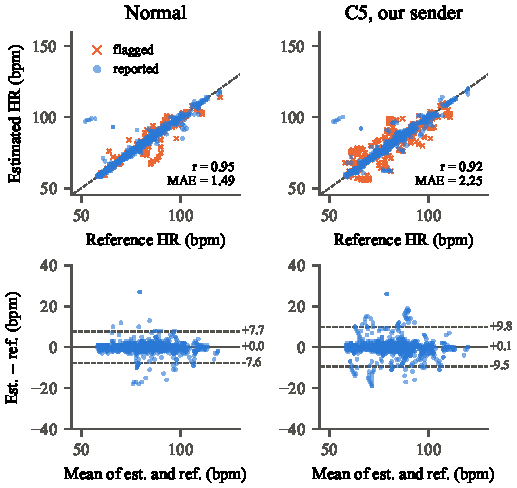
\includegraphics[width=\columnwidth]{figs/bland_altman.pdf}
\caption{Held-out subjects 61--80, proposed method. Top: estimated against reference HR per 10\,s window
(crosses: windows flagged by the quality gate). Bottom: Bland--Altman plots for all windows (bias and
95\,\% limits of agreement).}
\label{fig:ba}
\end{figure}

\subsection{Where the gains come from}
Table~\ref{tab:ladder} adds one stage at a time on the development set. Viterbi tracking removes
isolated wrong peaks, cutting the normal-condition MAE from 7.15 to 5.35\bpm. Illumination cancellation
helps most at 50\,lux and over compressed links, but costs a little at 20\,lux. Codec-pattern removal
acts only on streams that contain B-frames, where it lowers the error from 16.6 to 12.3\bpm. The learned
branch gives the largest single gain: it cuts the error by 43--64\,\% in every unmasked condition
(normal 5.0$\to$2.2\bpm; default x264 12.3$\to$4.5\bpm). Turning the tracker's harmonic boost back on
makes every condition worse.

The mask gate did \textit{not} lower the pooled error on simulated masks (9.99 against 8.70\bpm{} for
whole-face POS with tracking and illumination cancellation). A likely reason is that the simulated mask
is a static texture with no pulse: averaging it into the face dilutes the pulse without adding a
competing signal, which favours whole-face POS. A real mask moves with breathing and speech. The gate still detects
the mask in 100\,\% of masked windows, with 0.9\,\% false alarms in other conditions (development set). That signal lets
the quality gate withhold unreliable windows instead of failing silently, as C7 requires. Better
compensation is planned for Round~2.

\subsection{Low-bandwidth operation (C5)}
\begin{table}[t]
\caption{What broke 10\,fps / 500\,kbps, and the fixes (found on development subjects).}
\label{tab:c5}
\centering
\footnotesize
\setlength{\tabcolsep}{3pt}
\begin{tabular}{L{2.75cm}L{2.2cm}L{2.7cm}}
\toprule
Cause & Symptom & Fix \\
\midrule
Default x264 repeats P\,B\,B\,B; each position quantises the face colour differently &
false peak at $10/4=2.5$\,Hz (150\bpm) & sender: no B-frames (\texttt{zerolatency}); receiver: phase regression \\
\addlinespace
Picking the frame nearest each 0.1\,s tick from jittery stamps gives an uneven 2/3/4-frame pattern; with 100\,Hz light this aliases into the band &
the same 150\bpm{} lock, even without B-frames & keep exactly every 3rd frame; smooth the stamps \\
\addlinespace
Face mesh refreshed every 3rd \textit{frame}: only 3.3\,Hz at 10\,fps & regions drift during motion &
refresh at ${\sim}10$\,Hz in real time \\
\addlinespace
Tracker harmonic boost & fast HR read at half rate & boost disabled \\
\bottomrule
\end{tabular}
\end{table}

\begin{figure}[t]
\centering
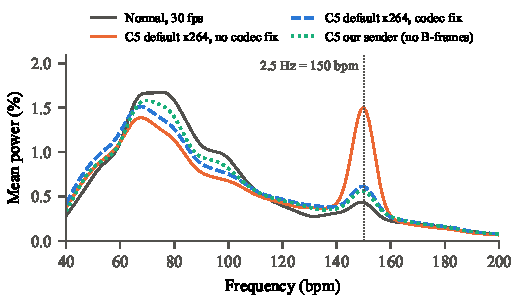
\includegraphics[width=\columnwidth]{figs/c5_spectra.pdf}
\caption{Mean normalised pulse spectrum over the 120 development videos. The default x264 stream at
10\,fps shows a peak at 150\bpm{} that does not depend on the subject's heart rate; codec-pattern removal
and our sender remove most of it.}
\label{fig:c5}
\end{figure}

The first run at 10\,fps / 500\,kbps failed in a characteristic way: many videos locked onto
150\bpm{} regardless of the true rate. Separating frame rate from bitrate on the development subjects
traced the failure to the four causes in Table~\ref{tab:c5}. Fig.~\ref{fig:c5} shows the main one.
Within $\pm3$\bpm{} of 150\bpm, the mean spectrum of default-x264 video holds 9.6\,\% of the power, against
2.9\,\% at 30\,fps. Codec-pattern removal lowers this to 4.1\,\%, and our sender to 3.8\,\%. The
remaining bump is common to all conditions and is not specific to compression. The fixes were frozen before the held-out sets were
scored. If the organisers' C5 videos are encoded with default settings, only the receiver-side fix
applies, giving 4.04\bpm{} on held-out subjects; with our sender settings the error is 2.25\bpm.

\subsection{Bystanders (C3)}
In all 40 held-out videos with a bystander, both faces were detected in every frame, and the target
was found in 99.9\,\% of frames. In every frame where both runs found the face, the target's colour trace
matched the single-person run within 5\,\%, so the tracker never switched to the bystander. The error is unchanged (1.44
against 1.49\bpm).

\subsection{Results by skin tone, age and sex (C2, C6)}\label{sec:strata}
\begin{table}[t]
\caption{Normal condition by subgroup: 80 subjects (1--60 out-of-fold, 61--80 held-out). MAE in bpm;
$\Delta$ is the difference from the pooled MAE.}
\label{tab:strata}
\centering
\footnotesize
\setlength{\tabcolsep}{3.2pt}
\begin{tabular}{lcccccc}
\toprule
Group & Subj. & MAE & $\Delta$ & ${\le}5$ (\%) & Reported (\%) & MAE rep. \\
\midrule
\tablerows{tables/strata.tex}
\bottomrule
\end{tabular}
\end{table}

Table~\ref{tab:strata} follows the brief's ITA-based stratification~\cite{chardon1991}. Measured ITA did not
predict error: the darkest third by ITA had an MAE of 1.84\bpm, against 2.03\bpm{} overall. However,
the absolute ITA values cannot be trusted. Because the webcam exposes faces dimly ($L^*\approx40$), the
measured ITA ranges from $-59^\circ$ to $+8^\circ$, which would put every subject in Fitzpatrick V--VI.
We therefore report relative thirds only. Proper C2 claims need colour-calibrated video and a dataset
with genuinely dark skin; we plan both for Round~2.

The four subjects aged 63--78 had an MAE of 0.38\bpm, and all their windows were reported. That
supports C6, but the group is far too small to establish it. The 30--59 group's error comes from a single
subject (age 54, MAE 20.1\bpm). In that subject the pulse is barely present in any region: about
10\,\% of the spectral power lies at the true rate, against 30--40\,\% normally. The gate withholds
65\,\% of those windows.

\subsection{Cross-dataset test on UBFC-rPPG}
\begin{table*}[t]
\caption{Cross-dataset results: UBFC-rPPG DATASET\_2 (42 subjects, whole videos, 2390 windows per condition), run
with the system frozen on MCD-rPPG subjects 1--60; nothing was retrained or re-tuned. Columns as in
Table~\ref{tab:heldout}.}
\label{tab:ubfc}
\centering
\footnotesize
\setlength{\tabcolsep}{3.4pt}
\begin{tabular}{lcccccccccc}
\toprule
 & \multicolumn{3}{c}{MAE, all windows} & \multicolumn{4}{c}{Proposed, all windows} & \multicolumn{3}{c}{Proposed, reported windows} \\
\cmidrule(lr){2-4}\cmidrule(lr){5-8}\cmidrule(lr){9-11}
Condition & POS & Classical & Proposed & RMSE & $r$ & BA bias [95\,\% LoA] & ${\le}5$\bpm{} (\%) & Reported (\%) & MAE & ${\le}5$\bpm{} (\%) \\
\midrule
\tablerows{tables/ubfc.tex}
\bottomrule
\end{tabular}
\end{table*}

To check that the system works beyond the data it was built on, we ran it unchanged on UBFC-rPPG
(Table~\ref{tab:ubfc}). Under normal conditions the MAE is 0.85\bpm{} ($r=0.99$, Bland--Altman bias
$+0.10$\bpm, limits $-3.9$ to $+4.1$\bpm), and only one of the 42 subjects has an MAE above 5\bpm{}
(5.3\bpm). Every simulated condition except low bandwidth stays below 1\bpm. That includes masks
(0.85\bpm): the mask was drawn and detected in every window of all 42 videos, but these faces keep a
strong pulse on the forehead and upper cheeks. UBFC is easier than MCD for every method (POS:
0.91\bpm), since its faces are well lit and the video is uncompressed. The learned branch adds little
here, but it does not hurt.

Low bandwidth is the exception. With our sender the MAE is 3.24\bpm{} (POS 9.15\bpm). With default
x264 settings the classical branch fails (32.7\bpm). In 25 of the 28 subjects whose heart rate averages
90\bpm{} or more, it locks onto 43--85\bpm, while the four subjects below 75\bpm{} average 2.6\bpm. We
have not yet confirmed the mechanism. One candidate is that at 500\,kbps the B-frames carry little new
colour information, which lowers the effective sampling rate of the colour signal. The learned branch
recovers part of the loss (fused 10.0\bpm), and the quality gate withholds 45\,\% of those windows. This
reinforces the main C5 lesson: at 10\,fps, the sender's encoder settings decide whether HR survives.

\pending{Results on a dataset with darker skin tones (Annexure~I), in a table like Table~\ref{tab:ubfc}.}

\subsection{Live operation and run time}
\begin{figure*}[t]
\centering
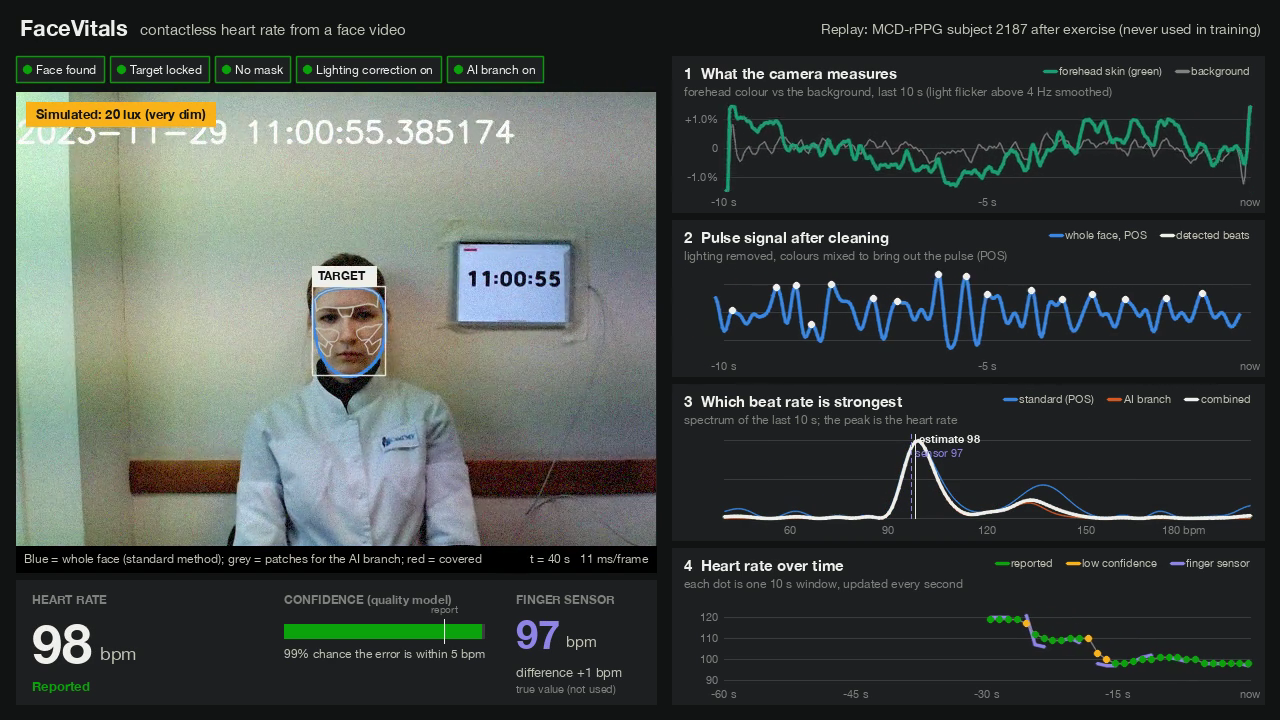
\includegraphics[width=0.84\textwidth]{figs/dashboard.png}
\caption{Live dashboard on a held-out MCD-rPPG subject~\cite{egorov2025} (CC\,BY\,4.0) under simulated
20\,lux. Left: the target face (whole-face region in blue, skin patches in grey) and the heart-rate card
with the quality gate's confidence and, for dataset replays, the finger-sensor reference. Right, in
pipeline order: forehead and background colour, the cleaned pulse with detected beats, the POS,
learned-branch and combined spectra, and the HR history (green: reported; orange: withheld).}
\label{fig:dashboard}
\end{figure*}

The live application (Fig.~\ref{fig:dashboard}) shows each stage as it runs, so a user can see why a
reading is reported or withheld. It uses the causal tracker and applies the quality gate to the newest
window. We replayed a held-out subject for 92\,s, switching to simulated 20\,lux and then to a mask
part-way through. The live error was 1.3\bpm, and 81\,\% of readings were reported.

On one Apple M3 Pro process, the front end (detection, mesh and region sampling) takes 5.5\,ms per
frame at 30\,fps and 13.1\,ms per frame at 10\,fps, where the mesh runs on every frame. Each HR update
takes 11.6\,ms, including the learned branch, and the online tracker step is negligible. With one
update per second, the pipeline uses about 18\,\% of one core at 30\,fps and 14\,\% at 10\,fps, so it
runs in real time on a laptop. We expect it to fit a Raspberry Pi~5, which has four cores, but have not
measured it yet. \pending{measured Raspberry Pi 5 timings}

% --------------------------------------------------------------------------------------------
\begin{table*}[t]
\caption{Round 1 constraint compliance. ``Sim.'' means simulated with the procedure in Section~\ref{sec:sim}.
Evidence gives the MAE in bpm on MCD-rPPG held-out subjects and, after the slash, on UBFC-rPPG.}
\label{tab:compliance}
\centering
\footnotesize
\begin{tabular}{L{0.5cm}L{3.6cm}L{5.0cm}L{5.9cm}L{1.0cm}}
\toprule
 & Specification & How it is addressed & Evidence: MAE, MCD held-out / UBFC & Status \\
\midrule
C1 & ${\le}50$\,lux at the face & illumination cancellation against background; learned branch; quality gate &
50\,lux: 2.14 / 0.90; 20\,lux: 2.38 / 0.95 (POS at 20\,lux: 7.49 / 1.51) & sim. \\
C2 & Fitzpatrick I--VI, per-type error & skin colour excluded from the gate; ITA stratification &
no trend with measured ITA; absolute ITA unreliable (Section~\ref{sec:strata}) & partial \\
C3 & track one target among several faces & detector + IoU tracker; mesh on the target only &
no identity switches in 40 videos; 1.44 / 0.85 & sim. \\
C4 & ${\le}640{\times}480$; QVGA stress case & everything runs at VGA; QVGA tested &
VGA baseline 1.49 / 0.85; QVGA 1.73 / 0.88 & sim. \\
C5 & ${\le}10$\,fps, ${\le}500$\,kbps; offline mode & sender without B-frames; codec-pattern removal; on-device pipeline &
our sender 2.25 / 3.24; default x264 4.04 / 10.04 & sim. \\
C6 & ages 60--70+, reported separately & no special handling &
4 subjects aged 63--78: MAE 0.38 (dev., out-of-fold) & partial \\
C7 & ${\ge}40$\,\% of lower face covered & mask detection; switch to upper patches; quality gate &
8.56 / 0.85; detected in every masked window; MCD: 37\,\% reported at 1.25 & sim. \\
\bottomrule
\end{tabular}
\end{table*}

\section{Compliance and Deliverables}
Table~\ref{tab:compliance} summarises the constraints. Five (C1, C3, C4, C5, C7) are addressed and
quantified on two datasets, and two (C2, C6) are reported in a preliminary form. \texttt{process\_round1.py} produces the Round~1
package in \texttt{/Round1\_Baseline/}: \texttt{Round1\_Baseline\_None.mat} (variables
\texttt{facial\_video}, \texttt{roi\_data}, \texttt{reference\_signal}, \texttt{processed\_signal},
\texttt{metrics} and \texttt{params}), \texttt{target\_video.mp4}, \texttt{reference\_signal.csv} and
\texttt{processed\_output.csv}. For each window it also writes $p_w$ and whether the window was
reported. \pending{store raw RGB frames in \texttt{facial\_video} (currently 72$\times$72 face crops) and fill lux, distance and
Fitzpatrick type in \texttt{params} for any recording that has them}.

\textit{Data and ethics.} Round~1 uses only public data: MCD-rPPG (CC\,BY\,4.0) and UBFC-rPPG, which its
authors share for research use and ask to be cited. Following the UBFC readme, no UBFC face images
appear in this report. We collected no new human data, so no IRB approval was needed for this round. \pending{if the team
records its own videos for Round~2, attach IRB approval and consent forms}. All code was written from
scratch, without third-party rPPG code, to avoid licence conflicts.

\section{Limitations and Round 2 Plan}
\begin{itemize}
\item Low light, masks and bystanders are simulated, and both datasets are indoor recordings of mostly
young adults. The next step is real recordings: real low-light video, a darker-skin dataset from
Annexure~I and, if possible, the organisers' hospital data.
\item Default H.264 at 10\,fps and 500\,kbps fails for fast heart rates (UBFC). We will test the
B-frame hypothesis and, if it holds, recommend no-B-frame encoding as part of the system.
\item C2 needs colour-calibrated skin-tone measurement (for example, a grey card) and per-type tolerances
set before testing.
\item Simulated masks: the learned branch is not yet trained on masked faces. We will train it with mask
augmentation and test against real masks.
\item Very weak pulses, such as the 54-year-old subject above, are not recovered by any branch; the
system abstains on them instead.
\item Talking and smiling. Our benchmarks score the first 40\,s of each video, while subjects sit still.
Later in one held-out video, where the subject smiles and moves, the live error rose to 13\bpm. Two thirds
of those readings were withheld, but one wrong reading (79 against 123\bpm) passed the gate. Motion
features for the gate and motion-robust regions are planned.
\item Round~2 (SpO$_2$): the same front end and regions give the per-channel AC/DC ratios needed for
ratio-of-ratios estimation. The quality gate will be extended to SpO$_2$.
\end{itemize}

\section{Conclusion}
A classical rPPG core, cleaned of codec and illumination artefacts, fused with a very small learned
branch and protected by a quality gate, estimates heart rate from low-quality facial video. On held-out
subjects, its error is 1.4--2.4\bpm{} under normal conditions and under simulated low light, low
resolution, bystanders and low-bandwidth streaming. Run unchanged on a second dataset (UBFC-rPPG), it
reaches 0.85\bpm. The biggest
practical lesson concerns C5: at 10\,fps the encoder's frame structure, not only its bitrate, decides
whether the pulse survives, and a single encoder setting removes most of the damage. Code, trained models and every result table are
reproducible from the accompanying scripts.

\begin{thebibliography}{99}
\bibitem{verkruysse2008} W.~Verkruysse, L.~O. Svaasand, and J.~S. Nelson, ``Remote plethysmographic imaging using ambient light,'' \textit{Opt. Express}, vol.~16, no.~26, pp. 21434--21445, 2008.
\bibitem{poh2010} M.-Z. Poh, D.~J. McDuff, and R.~W. Picard, ``Non-contact, automated cardiac pulse measurements using video imaging and blind source separation,'' \textit{Opt. Express}, vol.~18, no.~10, pp. 10762--10774, 2010.
\bibitem{dehaan2013} G.~de~Haan and V.~Jeanne, ``Robust pulse rate from chrominance-based rPPG,'' \textit{IEEE Trans. Biomed. Eng.}, vol.~60, no.~10, pp. 2878--2886, 2013.
\bibitem{wang2017} W.~Wang, A.~C. den Brinker, S.~Stuijk, and G.~de~Haan, ``Algorithmic principles of remote PPG,'' \textit{IEEE Trans. Biomed. Eng.}, vol.~64, no.~7, pp. 1479--1491, 2017.
\bibitem{li2014} X.~Li, J.~Chen, G.~Zhao, and M.~Pietik\"ainen, ``Remote heart rate measurement from face videos under realistic situations,'' in \textit{Proc. IEEE CVPR}, 2014, pp. 4264--4271.
\bibitem{chen2018deepphys} W.~Chen and D.~McDuff, ``DeepPhys: Video-based physiological measurement using convolutional attention networks,'' in \textit{Proc. ECCV}, 2018, pp. 349--365.
\bibitem{yu2019physnet} Z.~Yu, X.~Li, and G.~Zhao, ``Remote photoplethysmograph signal measurement from facial videos using spatio-temporal networks,'' in \textit{Proc. BMVC}, 2019.
\bibitem{liu2023efficientphys} X.~Liu, B.~Hill, Z.~Jiang, S.~Patel, and D.~McDuff, ``EfficientPhys: Enabling simple, fast and accurate camera-based cardiac measurement,'' in \textit{Proc. IEEE/CVF WACV}, 2023, pp. 5008--5017.
\bibitem{liu2023toolbox} X.~Liu \textit{et al.}, ``rPPG-Toolbox: Deep remote PPG toolbox,'' in \textit{Proc. NeurIPS Datasets and Benchmarks Track}, 2023.
\bibitem{mcduff2017} D.~J. McDuff, E.~B. Blackford, and J.~R. Estepp, ``The impact of video compression on remote cardiac pulse measurement using imaging photoplethysmography,'' in \textit{Proc. IEEE Int. Conf. Automatic Face \& Gesture Recognition (FG)}, 2017, pp. 63--70.
\bibitem{nowara2020} E.~M. Nowara, D.~McDuff, and A.~Veeraraghavan, ``A meta-analysis of the impact of skin tone and gender on non-contact photoplethysmography measurements,'' in \textit{Proc. IEEE/CVF CVPR Workshops}, 2020, pp. 284--285.
\bibitem{geifman2017} Y.~Geifman and R.~El-Yaniv, ``Selective classification for deep neural networks,'' in \textit{Proc. NeurIPS}, 2017, pp. 4878--4887.
\bibitem{wu2023yunet} W.~Wu, H.~Peng, and S.~Yu, ``YuNet: A tiny millisecond-level face detector,'' \textit{Machine Intelligence Research}, vol.~20, no.~5, pp. 656--665, 2023.
\bibitem{kartynnik2019} Y.~Kartynnik, A.~Ablavatski, I.~Grishchenko, and M.~Grundmann, ``Real-time facial surface geometry from monocular video on mobile GPUs,'' in \textit{Proc. IEEE/CVF CVPR Workshops}, 2019.
\bibitem{egorov2025} K.~Egorov, S.~Botman, P.~Blinov, G.~Zubkova, A.~Ivaschenko, A.~Kolsanov, and A.~Savchenko, ``Gaze into the heart: A multi-view video dataset for rPPG and health biomarkers estimation,'' in \textit{Proc. 33rd ACM Int. Conf. Multimedia}, 2025, doi: 10.1145/3746027.3758255.
\bibitem{bland1986} J.~M. Bland and D.~G. Altman, ``Statistical methods for assessing agreement between two methods of clinical measurement,'' \textit{Lancet}, vol.~327, no.~8476, pp. 307--310, 1986.
\bibitem{chardon1991} A.~Chardon, I.~Cretois, and C.~Hourseau, ``Skin colour typology and suntanning pathways,'' \textit{Int. J. Cosmet. Sci.}, vol.~13, no.~4, pp. 191--208, 1991.
\bibitem{bobbia2019} S.~Bobbia, R.~Macwan, Y.~Benezeth, A.~Mansouri, and J.~Dubois, ``Unsupervised skin tissue segmentation for remote photoplethysmography,'' \textit{Pattern Recognit. Lett.}, vol.~124, pp. 82--90, 2019.
\end{thebibliography}

\end{document}
